\chapter{Implementasi dan Pengujian}
\label{chap:implementasipengujian}

Pada bab ini akan dibahas mengenai hasil implementasi dan pengujian dari Open Source Snake 360. Permainan ini dapat dimainkan pada \textit{link} ini : \url{https://generaldevilx.github.io/Snake360/}

\section{Implementasi}
Pada bagian ini akan dijelaskan mengenai lingkungan yang digunakan untuk membangun dan implementasi antarmuka dari Open Source Snake 360.

\subsection{Lingkungan Perangkat Keras}
Berikut adalah lingkungan perangkat keras yang digunakan dalam pembangunan permainan ini: 

\begin{enumerate}
	\item Perangkat : Laptop
	\item \textit{Processor} : Intel Core i5-7200U 2.5GHz
	\item RAM : 4.00 GB
	\item \textit{Video Card} : GeForce 930MX
	\item Monitor : 14"
	\item \textit{Storage} : 1TB
\end{enumerate}

Pada pengujian digunakan 1 buah perangkat \textit{mobile} berbasis \textit{Android} dan 1 buah perangkat \textit{desktop}. Berikut adalah lingkungan perangkat keras yang digunakan dalam pengujian permainan ini:

\textbf{Perangkat 1}
\begin{enumerate}
	\item Perangkat : Laptop
	\item \textit{Processor} : Intel Core i5-7200U 2.5GHz
	\item RAM : 4.00 GB
	\item \textit{Video Card} : GeForce 930MX
	\item Monitor : 14"
	\item \textit{Storage} : 1TB
\end{enumerate}

\textbf{Perangkat 2}
\begin{enumerate}
	\item Perangkat : SM-J730G
	\item \textit{Processor} : Exynos 7870 Octa 1600MHz Cortex-A53
	\item RAM : 3.00 GB
	\item \textit{Video Card} : Mali-T830
	\item Monitor : 5.5"
	\item \textit{Storage} : 32 GB
\end{enumerate}

\subsection{Lingkungan Perangkat Lunak}
Berikut adalah lingkungan perangkat lunak yang digunakan dalam pembangunan permainan ini:

\begin{enumerate}
	\item Sistem Operasi Laptop : Windows 10 64-bit
	\item Bahasa Pemrograman : \textit{Javascript}, HTML
	\item Sistem Operasi \textit{Smartphone} : Android Nougat v7.0
\end{enumerate}

\subsection{GitHub Hosting}
Open Source Snake 360 dapat dimainkan pada link: \url{https://generaldevilx.github.io/Snake360/} karena permainan ini sudah dihosting di GitHub. Dengan cara ini, orang lain dapat memainkan Open Source Snake 360 secara langsung dengan mengakses link tersebut. Sebelum hosting, pada repository harus terdapat halaman utama yaitu 'index.html'. Caranya adalah : buka repository kemudian pilih tab 'settings'. Sesudah itu, carilah bagian 'GitHub Pages' kemudian pada bagian source, klik dropdown list dan akan muncul list seperti pada Gambar~\ref{fig:hosting}. List tersebut adalah branch pada repository yang akan dihosting. Karena peneliti menggunakan branch master untuk membuat Open Source Snake 360, maka list pertama akan dipilih. Setelah itu, GitHub akan menyediakan link yang dapat diakses oleh orang lain yang hasilnya dapat dilihat pada Gambar~\ref{fig:hosting2}.

\begin{figure}[H]
	\centering  
	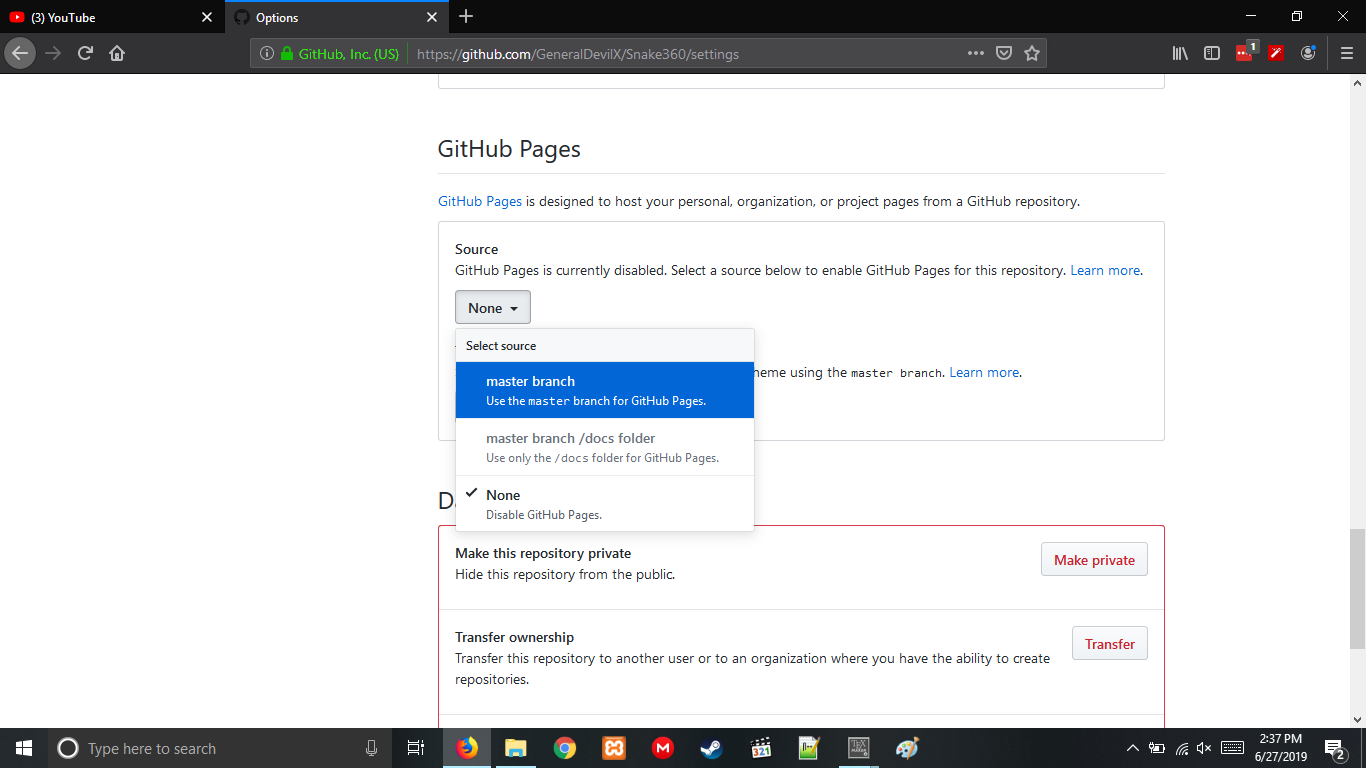
\includegraphics[scale=0.4]{hosting}  
	\caption[Tampilan memilih branch repository untuk dihosting]{Tampilan memilih branch repository untuk dihosting}
	\label{fig:hosting} 
\end{figure}

\begin{figure}[H]
	\centering  
	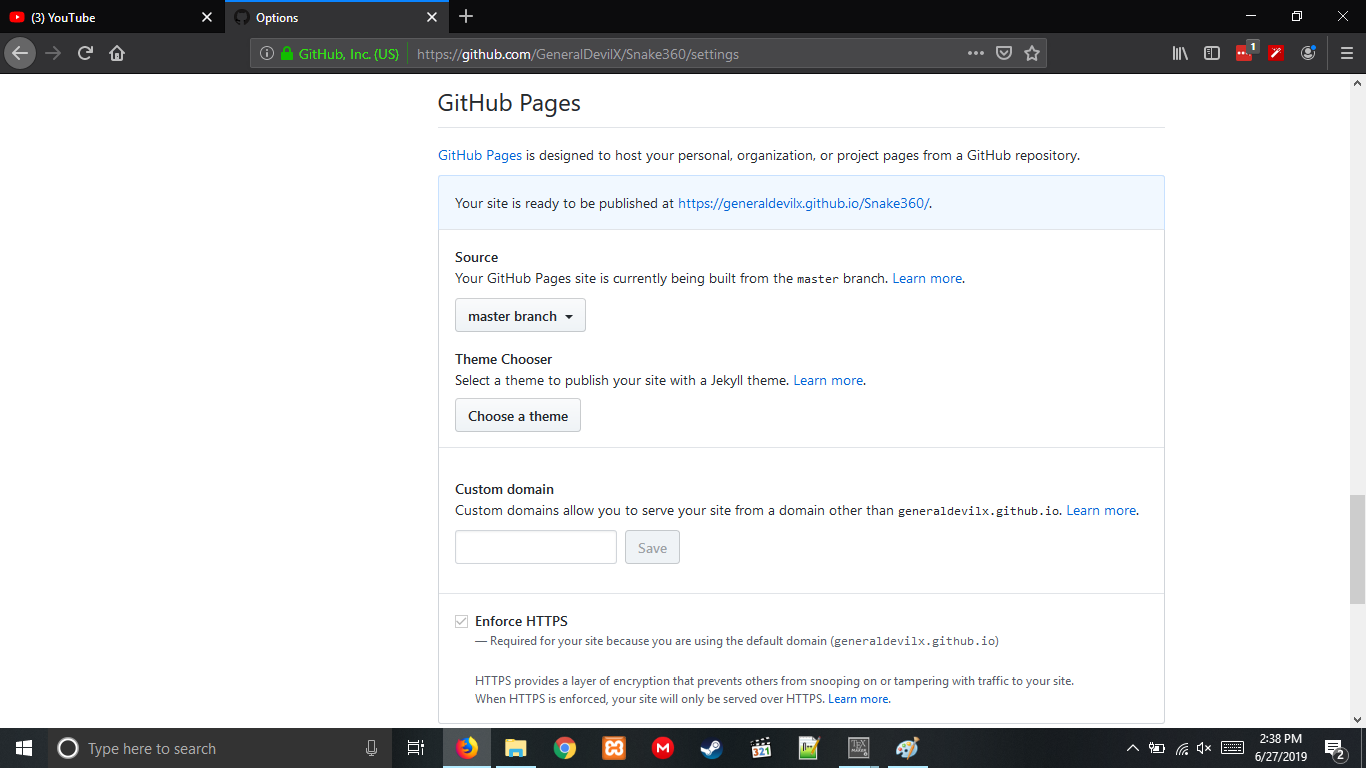
\includegraphics[scale=0.4]{hosting2}  
	\caption[Tampilan setelah melakukan hosting di GitHub]{Tampilan setelah melakukan hosting di GitHub}
	\label{fig:hosting2} 
\end{figure}

\subsection{Implementasi Antarmuka}
Pada subbab ini akan ditampilkan dan dijelaskan tampilan antarmuka dari Open Source Snake 360. 

\subsubsection{Tampilan Menu Utama}
Gambar~\ref{fig:GUIUtama} dan Gambar~\ref{fig:GUIUtamaAndroid} merupakan tampilan antarmuka menu utama pada \textit{desktop} dan \textit{smartphone}. Pada tampilan ini terdapat judul dari permainan, \textit{input} untuk mengisi \textit{level} labirin, kecepatan ular berbelok, kecepatan ular, dan tombol '\textit{Play Game}'. Jika pemain salah memasukkan data, maka terdapat pesan kesalahan yang ditandai dengan tulisan bewarna merah. Misal, pada Gambar~\ref{fig:GUIUtamaSalah} dan Gambar~\ref{fig:GUIUtamaSalahAndroid}, pemain salah memasukkan data untuk level labirin sehingga muncul pesan kesalahan bahwa \textit{input} yang dimasukkan salah.

\begin{figure}[H]
	\centering  
	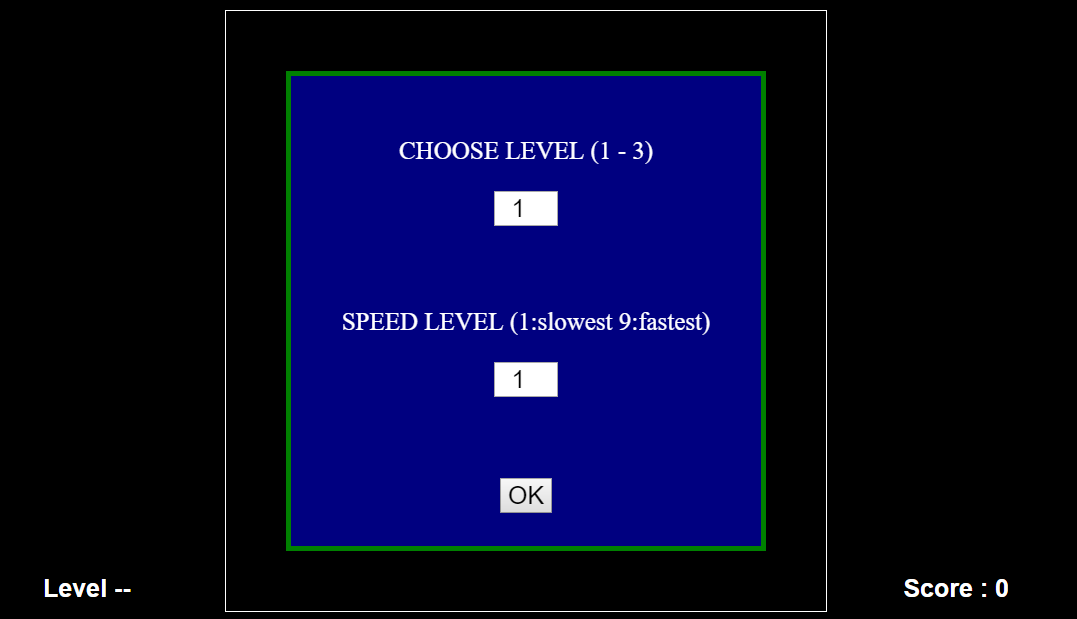
\includegraphics[scale=0.4]{GUIUtama}  
	\caption[Tampilan menu utama pada \textit{desktop}]{Tampilan menu utama pada \textit{desktop}}
	\label{fig:GUIUtama} 
\end{figure}

\begin{figure}[H]
	\centering  
	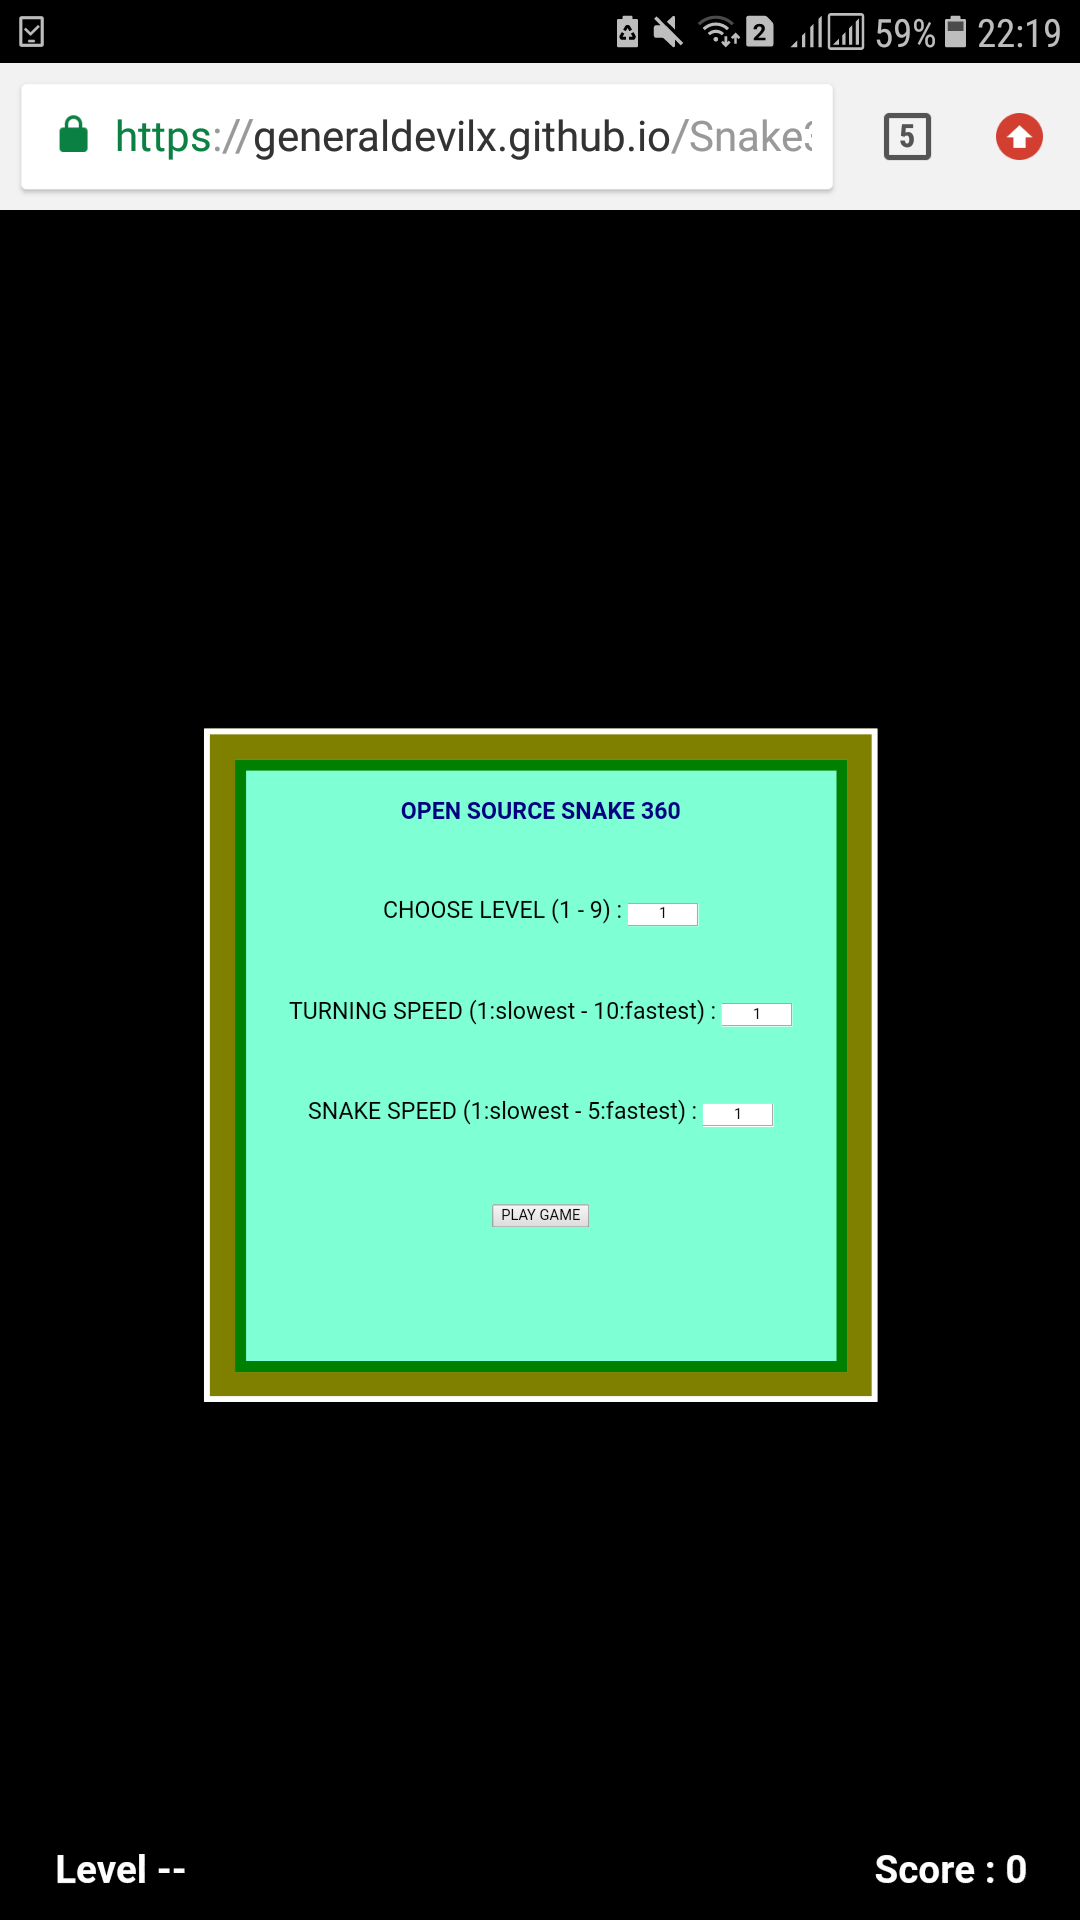
\includegraphics[scale=0.2]{GUIUtamaAndroid}  
	\caption[Tampilan menu utama pada \textit{smartphone}]{Tampilan menu utama pada \textit{smartphone}}
	\label{fig:GUIUtamaAndroid} 
\end{figure}

\begin{figure}[H]
	\centering  
	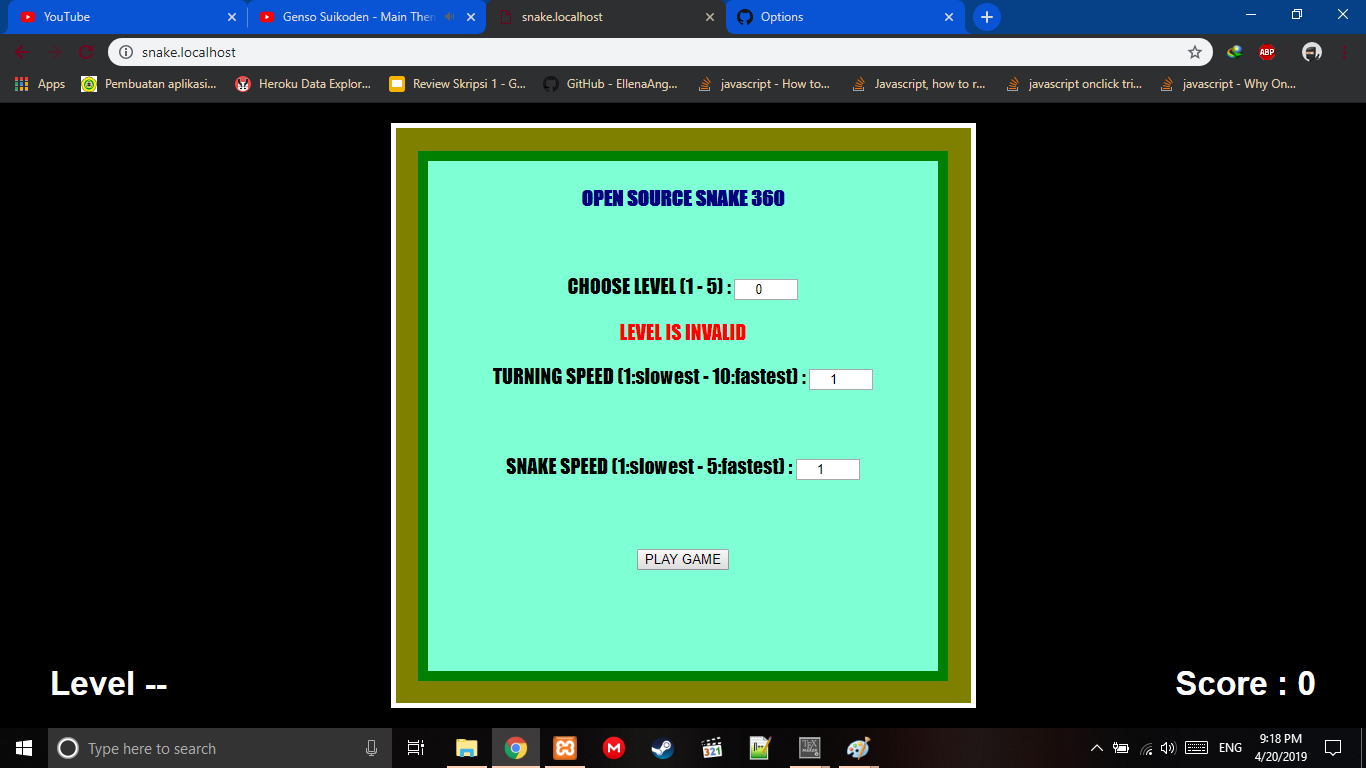
\includegraphics[scale=0.4]{GUIUtamaSalah}  
	\caption[Tampilan menu utama jika pemain salah memasukkan data \textit{level} labirin pada \textit{desktop}]{Tampilan menu utama jika pemain salah memasukkan data \textit{level} labirin pada \textit{desktop}}
	\label{fig:GUIUtamaSalah} 
\end{figure}

\begin{figure}[H]
	\centering  
	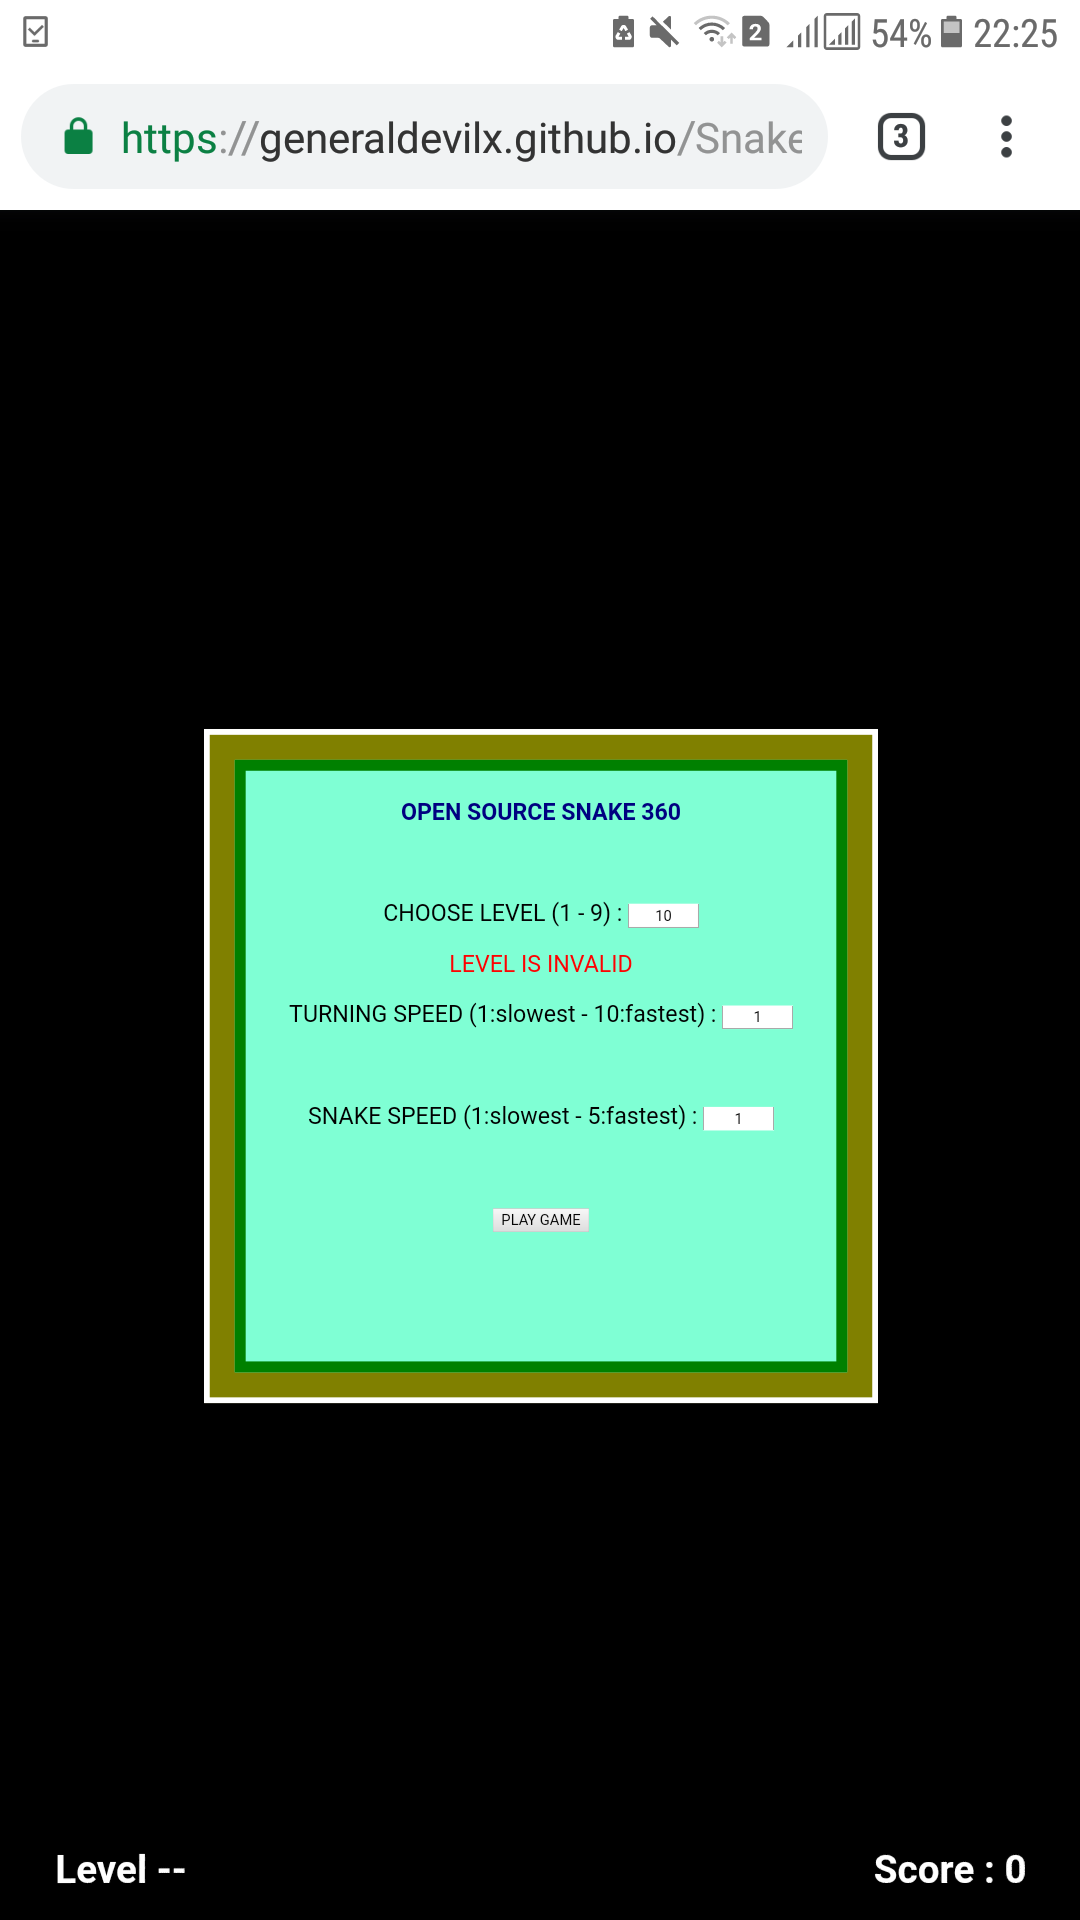
\includegraphics[scale=0.2]{GUIUtamaSalahAndroid}  
	\caption[Tampilan menu utama jika pemain salah memasukkan data \textit{level} labirin pada \textit{smartphone}]{Tampilan menu utama jika pemain salah memasukkan data \textit{level} labirin pada \textit{smartphone}}
	\label{fig:GUIUtamaSalahAndroid} 
\end{figure}

\subsubsection{Tampilan Bermain}
Gambar~\ref{fig:GUIBermain} dan Gambar~\ref{fig:GUIBermainAndroid} merupakan tampilan antarmuka mulai bermain pada \textit{desktop} dan \textit{smartphone}. Tampilan ini muncul apabila pemain memasukkan data level labirin, kecepatan ular berbelok dan kecepatan ular dengan benar dan menekan tombol "\textit{Play Game}". Pada tampilan ini terdapat ular yang dikontrol oleh pemain, dinding labirin, makanan ular, \textit{level} labirin dan skor yang didapat pemain.

\begin{figure}[H]
	\centering  
	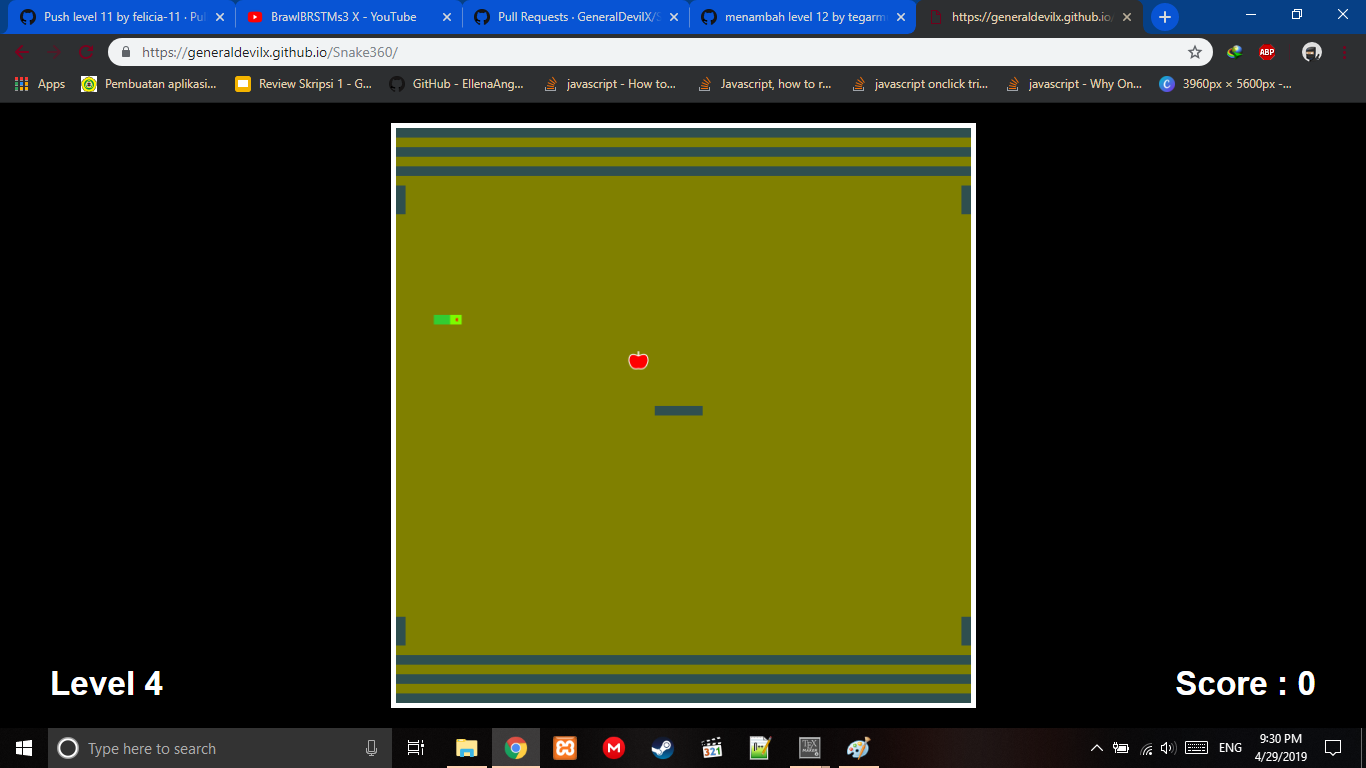
\includegraphics[scale=0.4]{GUIBermain}  
	\caption[Tampilan bermain pada \textit{desktop}]{Tampilan bermain pada \textit{desktop}}
	\label{fig:GUIBermain} 
\end{figure}

\begin{figure}[H]
	\centering  
	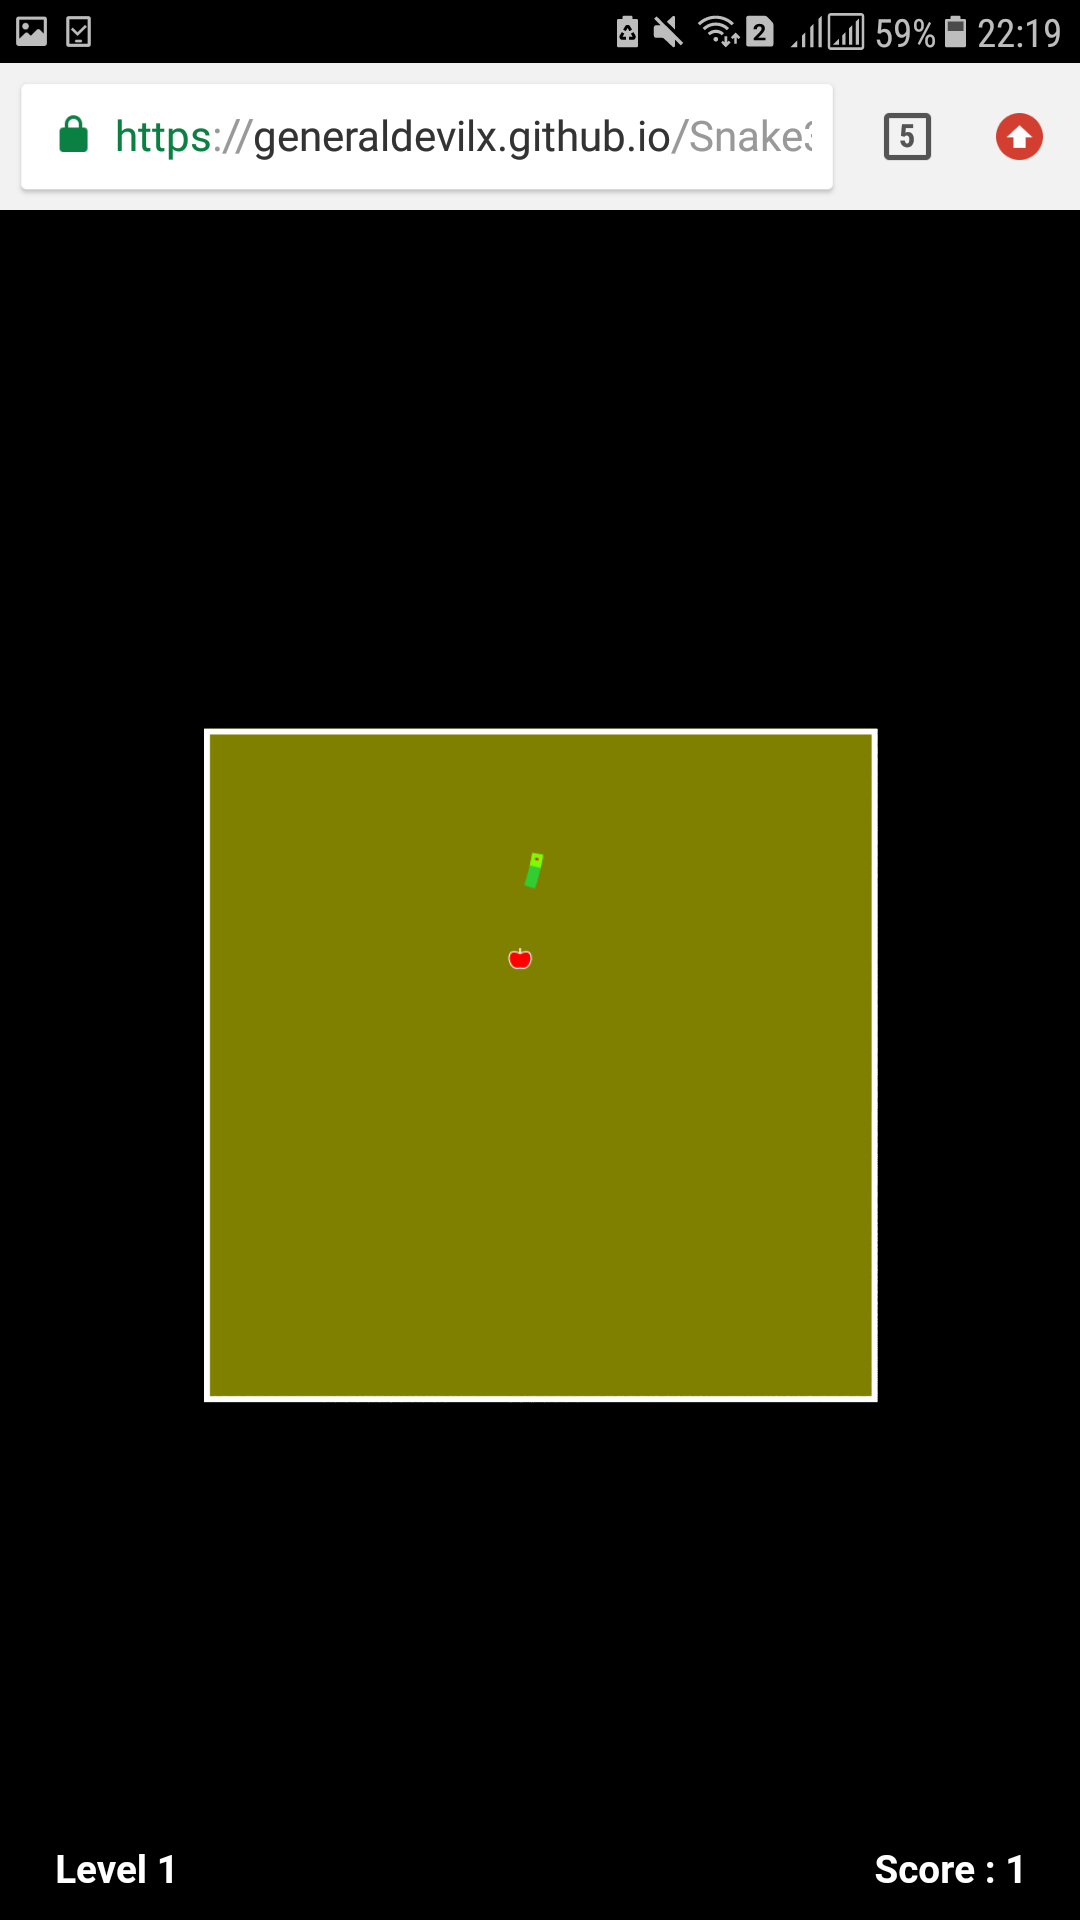
\includegraphics[scale=0.2]{GUIBermainAndroid}  
	\caption[Tampilan bermain pada \textit{smartphone}]{Tampilan bermain pada \textit{smartphone}}
	\label{fig:GUIBermainAndroid} 
\end{figure}

\subsubsection{Tampilan Permainan Berakhir}
Gambar~\ref{fig:GUIBerakhir} dan Gambar~\ref{fig:GUIBerakhirAndroid} merupakan tampilan antarmuka jika permainan berakhir pada \textit{desktop} dan \textit{smartphone}. Tampilan ini muncul apabila ular menabrak dinding labirin dan menabrak tubuhnya sendiri. Pemain akan diarahkan ke tampilan utama jika pemain menekan tombol '\textit{Enter}' pada tampilan ini. Karena pada smartphone tidak memiliki tombol 'Enter', maka pemain hanya memuat ulang/refresh halaman tersebut.

\begin{figure}[H]
	\centering  
	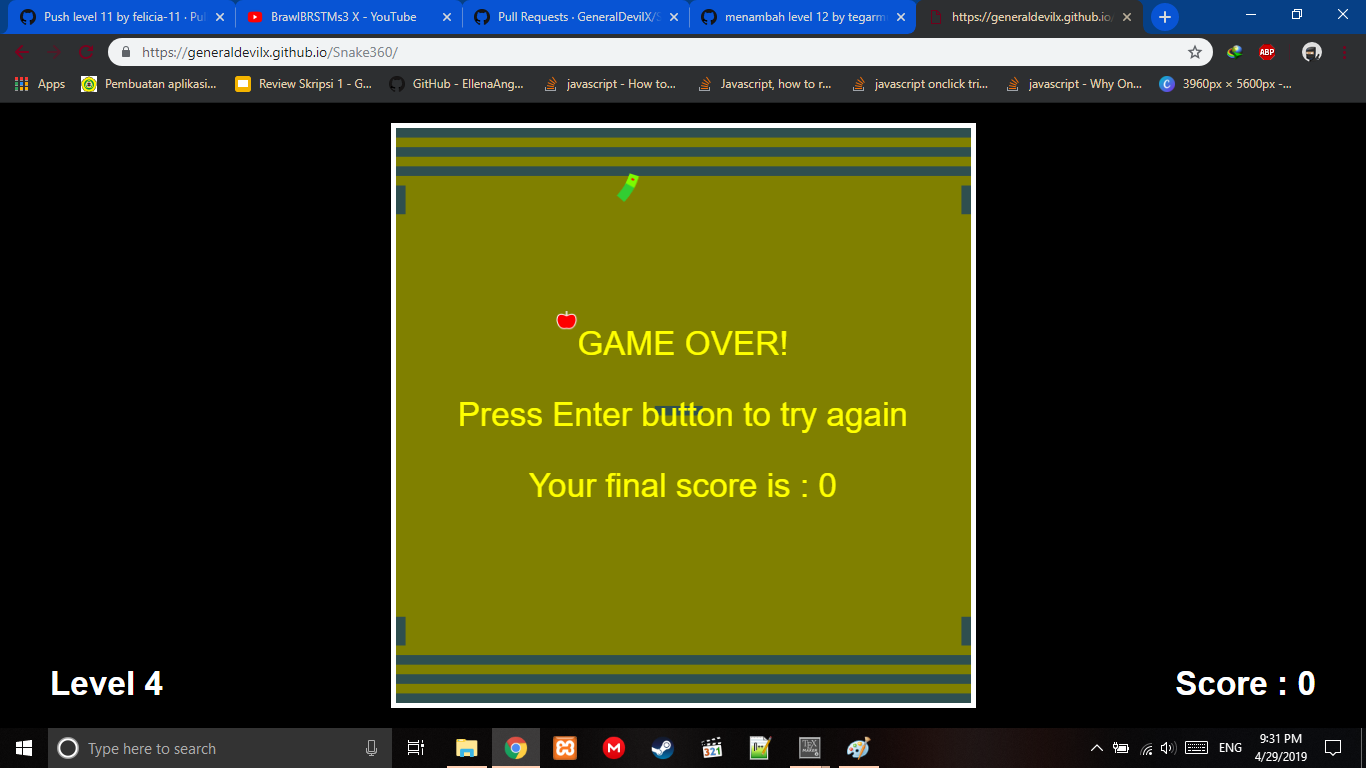
\includegraphics[scale=0.4]{GUIBerakhir}  
	\caption[Tampilan permainan berakhir pada desktop]{Tampilan permainan berakhir pada desktop}
	\label{fig:GUIBerakhir} 
\end{figure}

\begin{figure}[H]
	\centering  
	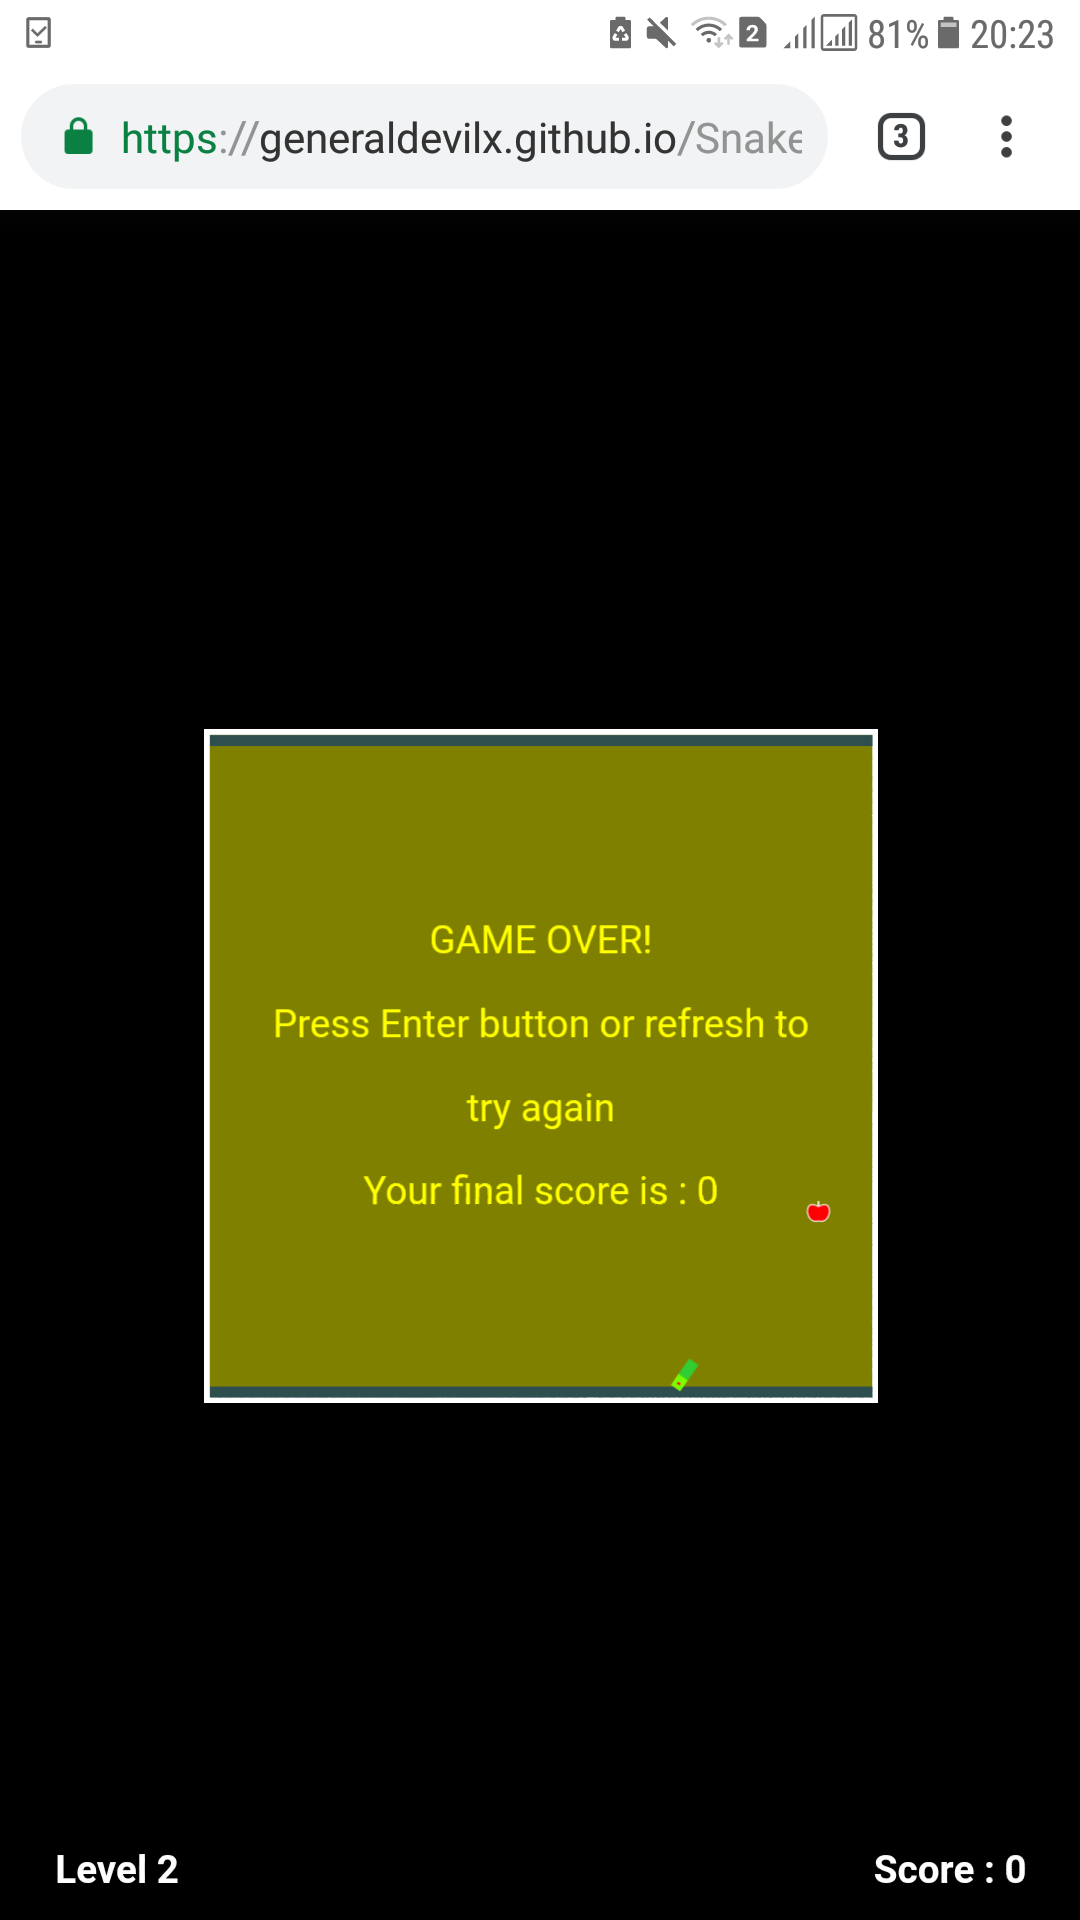
\includegraphics[scale=0.2]{GUIBerakhirAndroid}  
	\caption[Tampilan permainan berakhir pada smartphone]{Tampilan permainan berakhir smartphone}
	\label{fig:GUIBerakhirAndroid} 
\end{figure}

\section{Pengujian}
Pengujian terhadap permainan Open Source Snake 360 ini bertujuan untuk mengetahui apakah permainan yang dibangun sudah berjalan sesuai dengan rancangan. Pengujian yang dilakukan meliputi pengujian fungsional dan pengujian eksperimental. 

\subsection{Pengujian Fungsional}
Pengujian fungsional dilakukan untuk mengetahui tingkat keberhasilan perangkat lunak menjalankan fungsi-fungsi yang ada. Berikut akan ditunjukan pengujian pada tampilan: 

\begin{enumerate}
	\item Pengujian fungsionalitas pada tampilan menu utama.
	
	\begin{table}[H]
		\caption{Pengujian Fungsional pada Tampilan Menu Utama} \label{tab:table1}
		\begin{tabular}{| m{4cm} | m{6cm}  | m{4cm} |}
			\hline
			Kasus uji & Hasil yang diharapkan & Hasil uji \\ \hline
			Pemain memilih labirin dan kecepatan berbelok & Jika pemain salah memasukkan data level labirin, maka akan ditampilkan sebuah text bahwa data yang diisi tidak valid & Hasil pengujian sesuai dengan yang diharapkan\\ \hline
			Pada bagian pemilihan level labirin, terdapat jumlah labirin yang dapat dipilih oleh pemain & Jumlah labirin yang ditampilkan harus sesuai dengan jumlah labirin yang terdapat pada server & Hasil pengujian sesuai dengan yang diharapkan\\ \hline
			Pemain menekan tombol "Play Game" & Pemain akan diarahkan ke tampilan bermain. Kondisi untuk dapat memulai permainan adalah data level labirin, kecepatan berbelok dan kecepatan laju ular sudah valid. Posisi ular dan dinding labirin sesuai dengan level labirin yang dipilih. Posisi apel tidak berada di atas dinding labirin atau tubuh ular. & Umumnya, posisi apel tidak berada tepat di atas dinding labirin. Pada beberapa kasus, posisi apel tepat berada di atas dinding labirin.\\ \hline
		\end{tabular}
	\end{table}
	
	Berdasarkan tabel~\ref{tab:table1}, dapat disimpulkan bahwa kasus uji pada tampilan menu utama belum membawakan hasil sesuai dengan yang diharapkan ketika pemain menekan tombol "Play Game". Hal ini disebabkan karena pengecekan tabrakan antara apel dengan dinding labirin kurang akurat. 
	
	\item Pengujian fungsionalitas tampilan bermain pada \textit{desktop}.
	
	\begin{table}[H]
		\caption{Pengujian Fungsional Tampilan Bermain pada Desktop} \label{tab:table2}
		\begin{tabular}{| m{4cm} | m{6cm}  | m{4cm} |}
			\hline
			Kasus uji & Hasil yang diharapkan & Hasil uji \\ \hline
			Tombol arah kiri ditekan & Ular akan bergerak melawan arah jarum jam & Hasil pengujian sesuai dengan yang diharapkan\\ \hline
			Tombol arah kanan ditekan & Ular akan bergerak searah jarum jam & Hasil pengujian sesuai dengan yang diharapkan\\ \hline
			Ular memakan apel & Pemain akan mendapatkan skor & Hasil pengujian sesuai dengan yang diharapkan\\ \hline
			Ular menabrak dinding & Tampilan "\textit{game over}" akan muncul & Hasil pengujian sesuai dengan yang diharapkan\\ \hline
			Ular menabrak tubuh sendiri & Tampilan "\textit{game over}" akan muncul & Hasil pengujian sesuai dengan yang diharapkan\\ \hline 
			Ular mencapai sisi ujung labirin & Ular akan muncul di sisi ujung labirin yang berlawanan & Hasil pengujian sesuai dengan yang diharapkan\\ \hline
			Tombol arah kanan ditekan 9 kali dengan kecepatan sudut sebesar 10  & Ular akan bergerak ke bawah & Hasil pengujian sesuai dengan yang diharapkan\\ \hline
			Tombol arah kiri ditekan 9 kali dengan kecepatan sudut sebesar 10  & Ular akan bergerak ke atas & Hasil pengujian sesuai dengan yang diharapkan\\ \hline
		\end{tabular}
	\end{table}
	
	Berdasarkan tabel~\ref{tab:table2}, dapat disimpulkan bahwa kasus uji tampilan bermain pada desktop membawakan hasil sesuai dengan yang diharapkan.
	
	\item Pengujian fungsionalitas tampilan bermain pada \textit{smartphone}.
	
	\begin{table}[H]
		\caption{Pengujian Fungsional Tampilan Bermain pada \textit{Smartphone}} \label{tab:table3}
		\begin{tabular}{| m{4cm} | m{6cm}  | m{4cm} |}
			\hline
			Kasus uji & Hasil yang diharapkan & Hasil uji \\ \hline
			Bagian kiri layar ditekan & Ular akan bergerak melawan arah jarum jam & Ketika menekan layar lebih lama, akan muncul sebuah menu yang menginterupsi. Ular akan terus bergerak melawan arah jarum jam meskipun bagian kiri layar tidak ditekan sama sekali.\\ \hline
			Bagian kanan layar ditekan & Ular akan bergerak searah jarum jam & Ketika menekan layar lebih lama, akan muncul sebuah menu yang menginterupsi. Ular akan terus bergerak searah arah jarum jam meskipun bagian kanan layar tidak ditekan sama sekali.\\ \hline
			Ular memakan apel & Pemain akan mendapatkan skor & Hasil pengujian sesuai dengan yang diharapkan\\ \hline
			Ular menabrak dinding & Tampilan "\textit{game over}" akan muncul & Hasil pengujian sesuai dengan yang diharapkan\\ \hline
			Ular menabrak tubuh sendiri & Tampilan "\textit{game over}" akan muncul & Hasil pengujian sesuai dengan yang diharapkan\\ \hline 
			Ular mencapai sisi ujung labirin & Ular akan muncul di sisi ujung labirin yang berlawanan & Hasil pengujian sesuai dengan yang diharapkan\\ \hline
			Bagian kanan layar ditekan 9 kali dengan kecepatan sudut sebesar 10  & Ular akan bergerak ke bawah & Hasil pengujian sesuai dengan yang diharapkan\\ \hline
			Bagian kiri layar ditekan 9 kali dengan kecepatan sudut sebesar 10  & Ular akan bergerak ke atas & Hasil pengujian sesuai dengan yang diharapkan\\ \hline
		\end{tabular}
	\end{table}
	
	Berdasarkan tabel~\ref{tab:table3}, dapat disimpulkan bahwa kasus uji tampilan bermain pada \textit{smartphone} belum membawakan hasil sesuai dengan yang diharapkan. Hal ini dikarenakan \textit{web browser} pada  smartphone akan otomatis memunculkan menu jika layar \textit{smartphone} ditekan lebih lama.
	
	\item Pengujian fungsionalitas tampilan permainan berakhir
	
	\begin{table}[H]
		\caption{Pengujian Fungsional Tampilan Permainan Berakhir} \label{tab:table4}
		\begin{tabular}{| m{4cm} | m{6cm}  | m{4cm} |}
			\hline
			Kasus uji & Hasil yang diharapkan & Hasil uji \\ \hline
			Tombol "\textit{Enter}" ditekan (pada \textit{desktop}) atau pemain memuat ulang halaman (pada \textit{smartphone})& Pemain akan diarahkan ke tampilan menu utama & Hasil pengujian sesuai dengan yang diharapkan\\ \hline
		\end{tabular}
	\end{table}
	
	Berdasarkan tabel~\ref{tab:table4}, dapat disimpulkan bahwa kasus uji pada tampilan "game over" membawakan hasil sesuai dengan yang diharapkan. 
\end{enumerate}

\subsection{Pengujian Eksperimental}
Pada pengujian eksperimental akan diuji penambahan labirin oleh orang lain. Pada pengujian ini terdapat 5 orang yang akan menambahkan labirin menggunakan \textit{pull request GitHub}. Setiap penguji diminta untuk membaca \textit{file} \textit{readme} (lampiran ~\ref{lamp:B}) yang berisikan tentang cara menambah labirin. Berikut adalah hasil pengujian eksperimental : 

\begin{enumerate}
	\item Penguji 1 : EllenaAngelica\\
	Penguji 1 berhasil menambahkan labirin ke 6 dengan menggunakan \textit{pull request} seperti yang terlihat pada Gambar~\ref{fig:pullReq1}. \textit{Link} untuk \textit{file} teks yang dibuat penguji 1 :  \url{https://github.com/GeneralDevilX/Snake360/pull/3/files}. Gambar~\ref{fig:pengujian1} merupakan hasil pengujian menggunakan labirin yang dibuat oleh penguji 1. Pada Gambar~\ref{fig:pengujian1}, Penguji 1 membuat labirin yang sudah sesuai dengan besar \textit{canvas}. Namun posisi ular yang dimasukkan tidak sesuai. Penguji 1 menambahkan sebuah baris kosong di akhir \textit{file} tersebut sehingga menyebabkan permainan menjadi \textit{error}. Hal ini disebabkan karena pembacaan posisi ular selalu mengambil teks baris paling terakhir. Karena itu, peneliti harus memperbaiki labirin yang dibuat oleh penguji 1.
	
	\begin{figure}[H]
		\centering  
		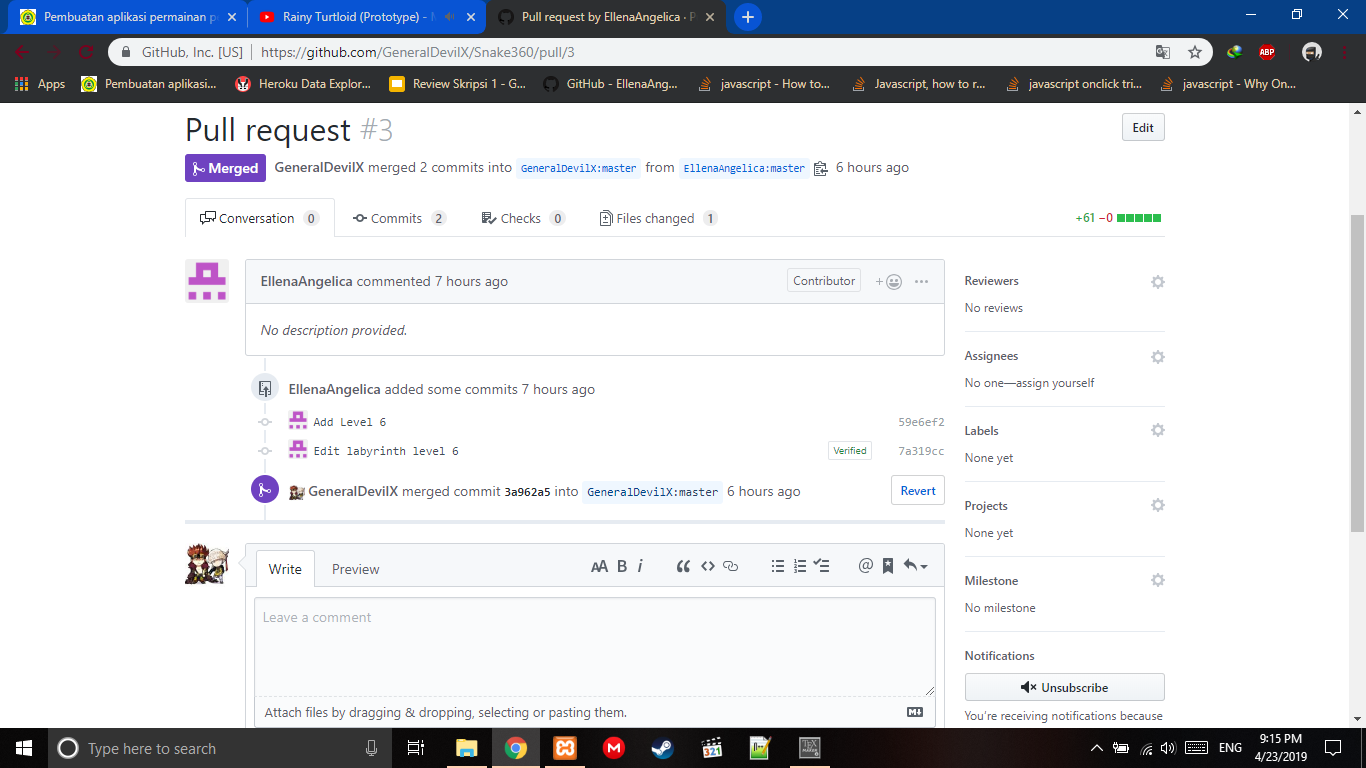
\includegraphics[scale=0.4]{pullReq1}  
		\caption[Tampilan hasil \textit{pull request} milik penguji 1]{Tampilan hasil \textit{pull request} milik penguji 1}
		\label{fig:pullReq1} 
	\end{figure}
	
	\begin{figure}[H]
		\centering  
		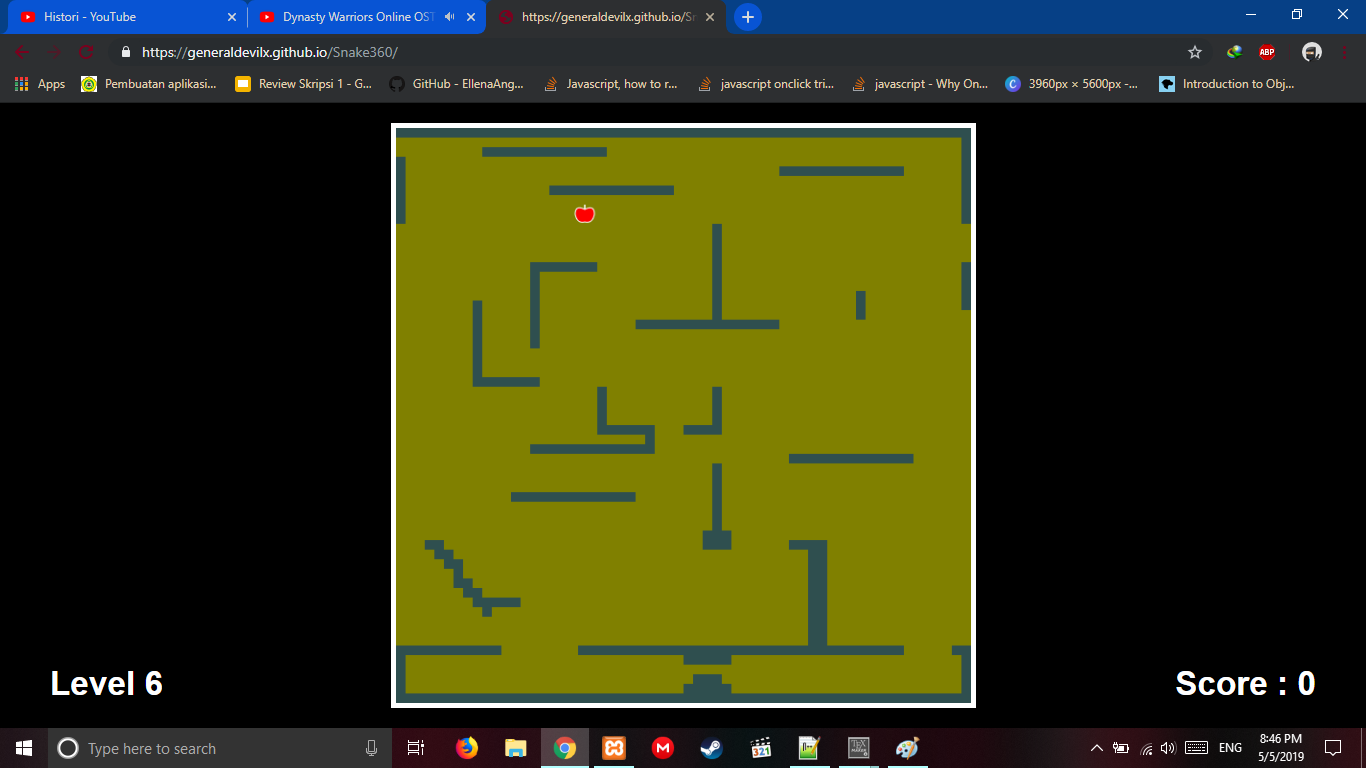
\includegraphics[scale=0.4]{pengujian1}  
		\caption[Tampilan pengujian labirin ke 6 yang dibuat oleh penguji 1]{Tampilan pengujian labirin yang dibuat oleh penguji 1}
		\label{fig:pengujian1} 
	\end{figure}	
	
	\item Penguji 2 : adamadamadamadamadam\\
	Penguji 2 berhasil menambahkan labirin ke 7, 8 dan 9 dengan menggunakan \textit{pull request} seperti yang terlihat pada Gambar~\ref{fig:pullReq2}. \textit{Link} untuk \textit{file} teks yang dibuat penguji 2 : \url{https://github.com/GeneralDevilX/Snake360/pull/2/files}. Penguji 2 membuat labirin ke 7 yang seluruhnya terdapat dinding dan memposisikan ular di koordinat (0,0). Selain itu, pada file teks labirin ke 7, labirin dibuat kurang dari 60 baris. Penguji 2 membuat labirin ke 7 dan labirin ke 8. Gambar~\ref{fig:pengujian2} merupakan hasil pengujian labirin ke 7.
	
	
	Ketiga labirin yang dibuat oleh penguji 2 tidak sesuai dengan besar \textit{canvas} sehingga tampilan menjadi seperti pada Gambar~\ref{fig:pengujian2}. Penguji 2 membuat labirin \textit{level} 7 dan 8 yang seluruhnya adalah dinding dan memposisikan ular di (0,0). Pada labirin level 9, penguji 2 menambahkan sebuah baris kosong di akhir \textit{file} sehingga menyebabkan permainan menjadi \textit{error}. Peneliti ingin memberitahukan penguji 2 bahwa labirin yang dibuat belum benar, tetapi terjadi sebuah kesalahan yaitu peneliti menekan tombol \textit{merge request}. Hal ini membuat peneliti harus memperbaiki labirin yang dibuat oleh penguji 2.
	
	\begin{figure}[H]
		\centering  
		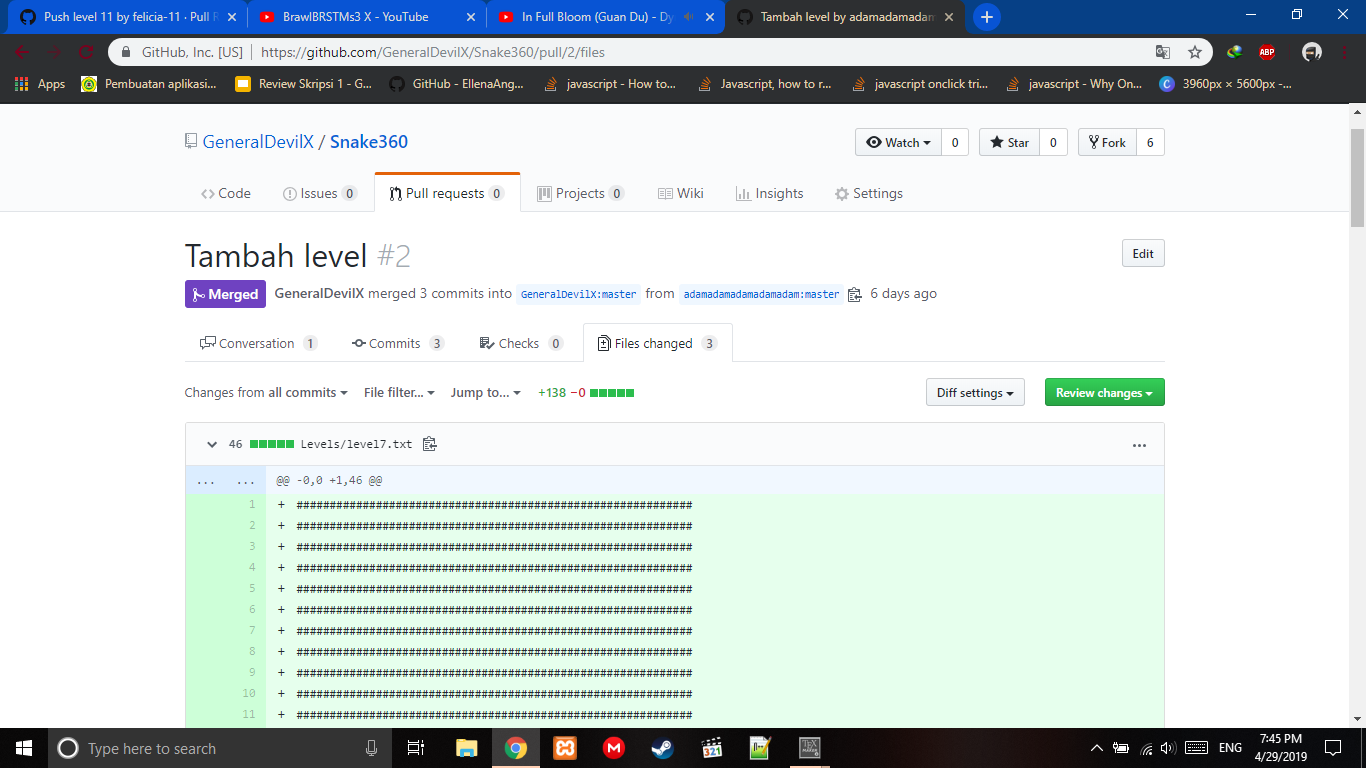
\includegraphics[scale=0.4]{pullReq2}  
		\caption[Tampilan hasil \textit{pull request} milik penguji 2]{Tampilan hasil \textit{pull request} milik penguji 2}
		\label{fig:pullReq2} 
	\end{figure}
	
	\begin{figure}[H]
		\centering  
		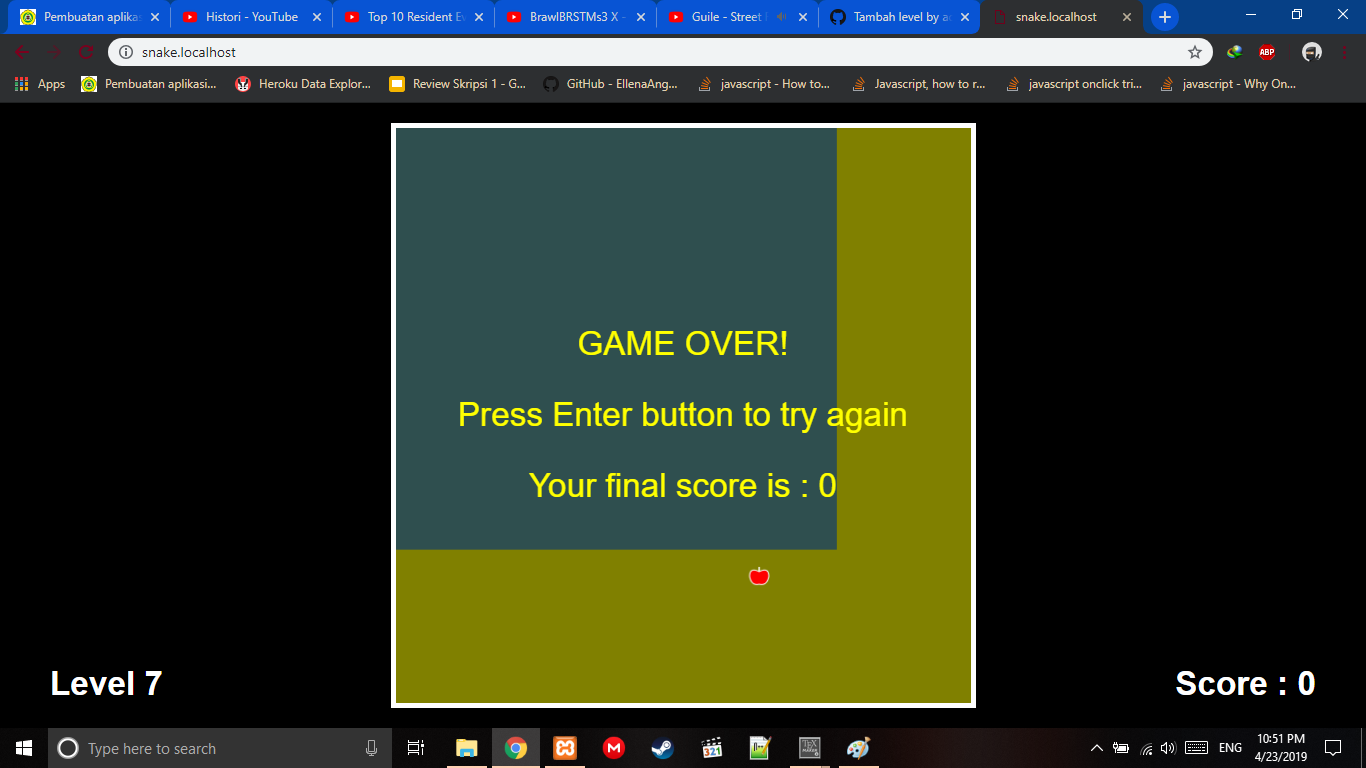
\includegraphics[scale=0.4]{pengujian2}
		\caption[Tampilan pengujian labirin ke 7 yang dibuat oleh penguji 2]{Tampilan pengujian labirin ke 7 yang dibuat oleh penguji 2}
		\label{fig:pengujian2} 
	\end{figure}
	
	\begin{figure}[H]
		\centering  
		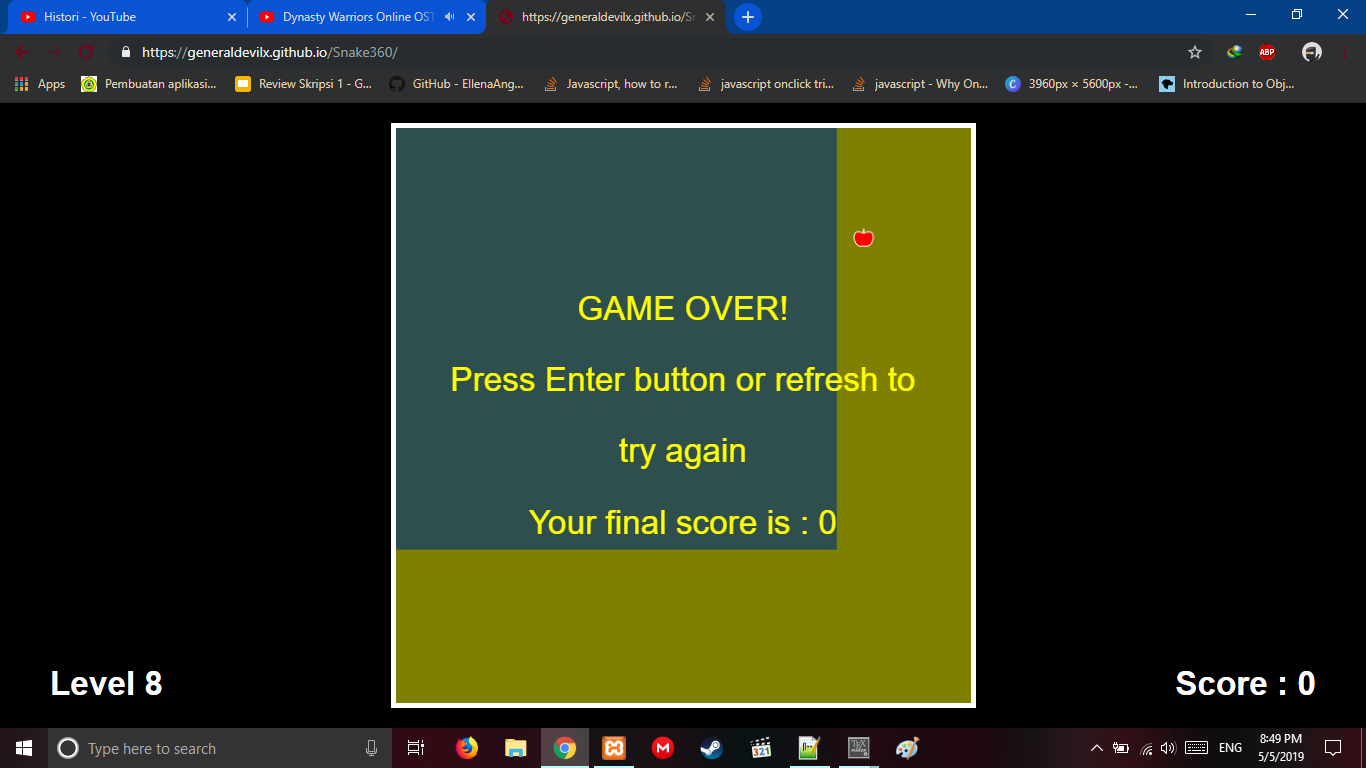
\includegraphics[scale=0.4]{pengujian2_2}  
		\caption[Tampilan pengujian labirin ke 8 yang dibuat oleh penguji 2]{Tampilan pengujian labirin ke 8 yang dibuat oleh penguji 2}
		\label{fig:pengujian2_2} 
	\end{figure}
	
	\begin{figure}[H]
		\centering  
		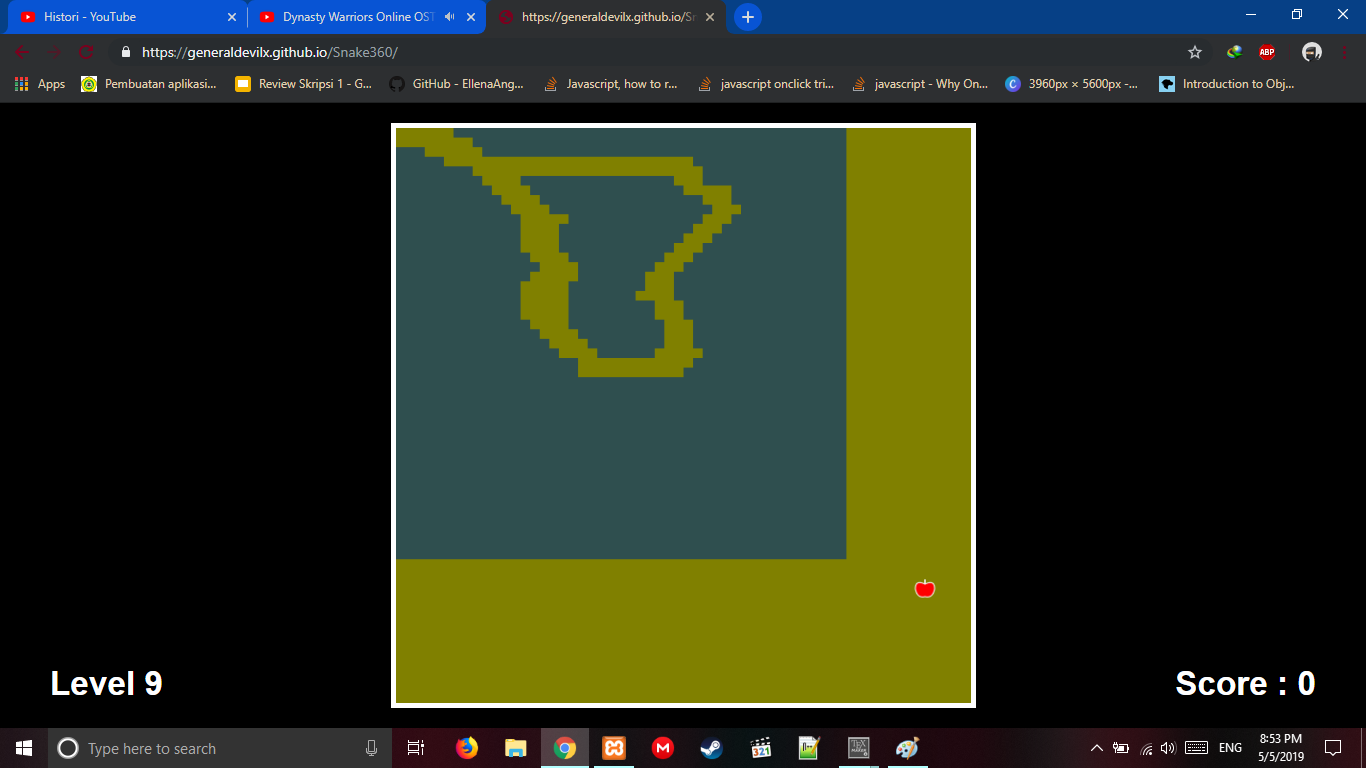
\includegraphics[scale=0.4]{pengujian2_3}  
		\caption[Tampilan pengujian labirin ke 9 yang dibuat oleh penguji 2]{Tampilan pengujian labirin ke 9 yang dibuat oleh penguji 2}
		\label{fig:pengujian2_3} 
	\end{figure}
	
	\item Penguji 3 : ThobyGitHub\\
	Penguji 3 berhasil menambahkan labirin \textit{level} 10 dengan menggunakan pull request seperti yang terlihat pada Gambar~\ref{fig:pullReq3}. \textit{Link} untuk \textit{file} teks yang dibuat penguji 3 : \url{https://github.com/GeneralDevilX/Snake360/pull/4/files}. Labirin yang dibuat oleh penguji 3 sudah sesuai ketentuan membuat labirin pada \textit{file readme}. Gambar~\ref{fig:pengujian3} merupakan tampilan labirin yang dibuat oleh penguji 3.
	
	\begin{figure}[H]
		\centering  
		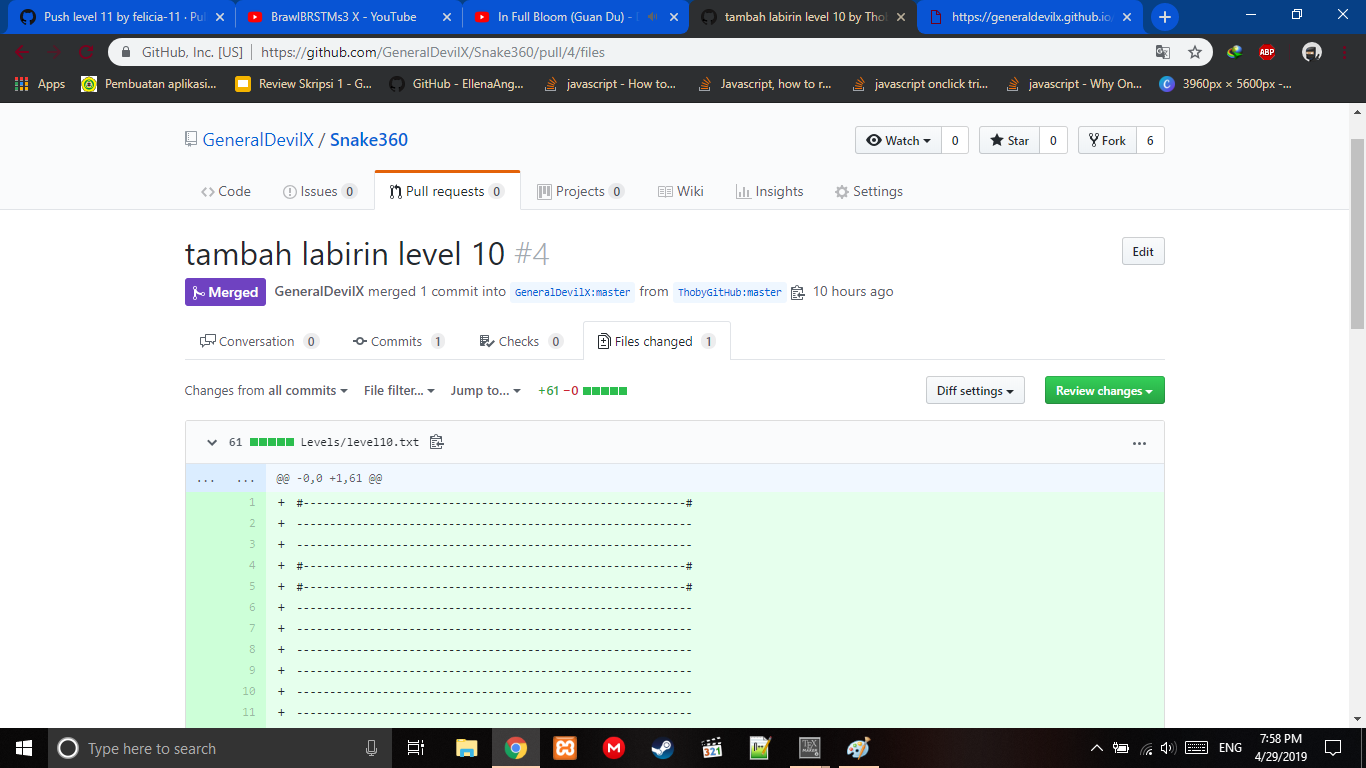
\includegraphics[scale=0.4]{pullReq3}  
		\caption[Tampilan hasil pull request milik penguji 3]{Tampilan hasil pull request milik penguji 3}
		\label{fig:pullReq3} 
	\end{figure}
	
	\begin{figure}[H]
		\centering  
		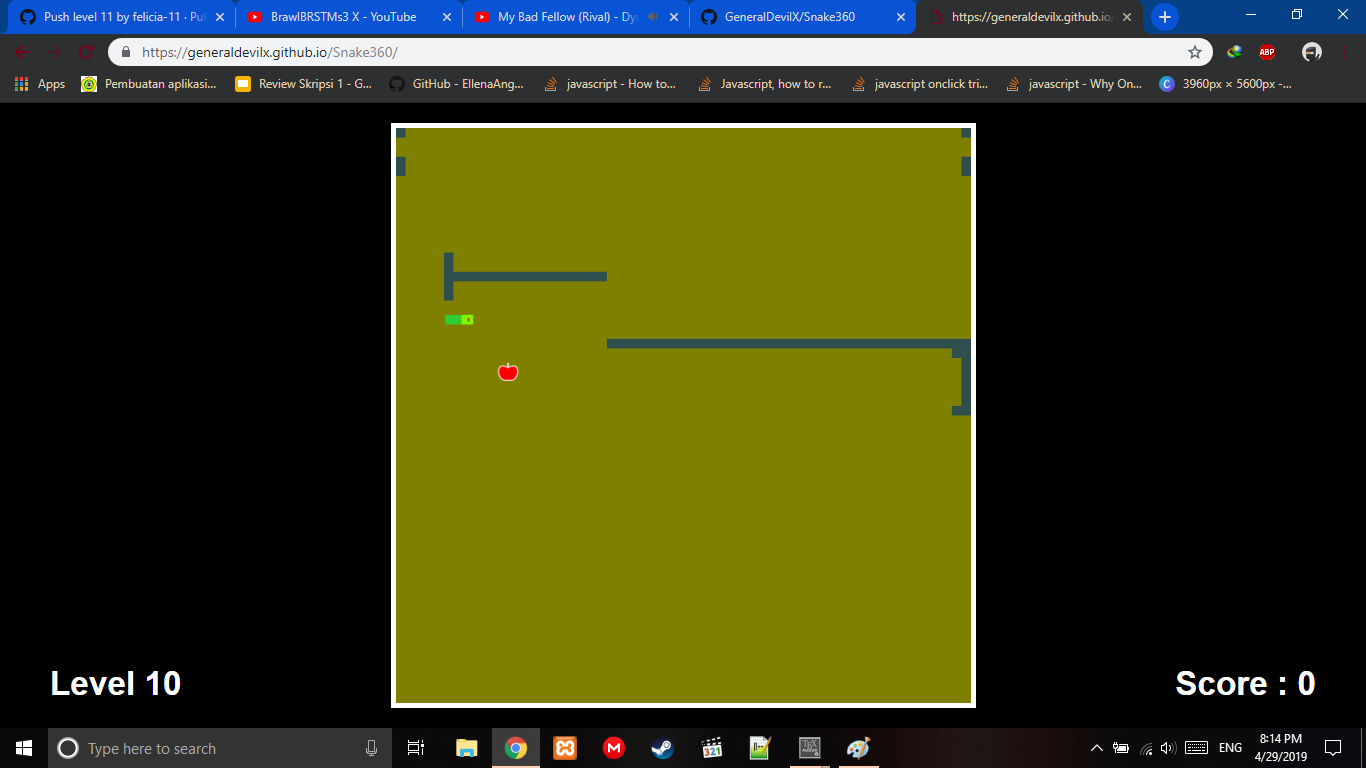
\includegraphics[scale=0.4]{pengujian3}  
		\caption[Tampilan pengujian labirin yang dibuat oleh penguji 3]{Tampilan pengujian labirin yang dibuat oleh penguji 3}
		\label{fig:pengujian3} 
	\end{figure}
	
	\item Penguji 4 : felicia-11\\
	Penguji 4 berhasil menambahkan labirin level 11 dengan menggunakan \textit{pull request} seperti yang terlihat pada Gambar~\ref{fig:pullReq4}. \textit{Link} untuk \textit{file} teks yang dibuat penguji 4 : \url{https://github.com/GeneralDevilX/Snake360/pull/6/files}. Labirin yang dibuat oleh penguji 4 sudah sesuai ketentuan membuat labirin pada \textit{file readme} sehingga tampilan menjadi seperti pada Gambar~\ref{fig:pengujian4}.
	
	\begin{figure}[H]
		\centering  
		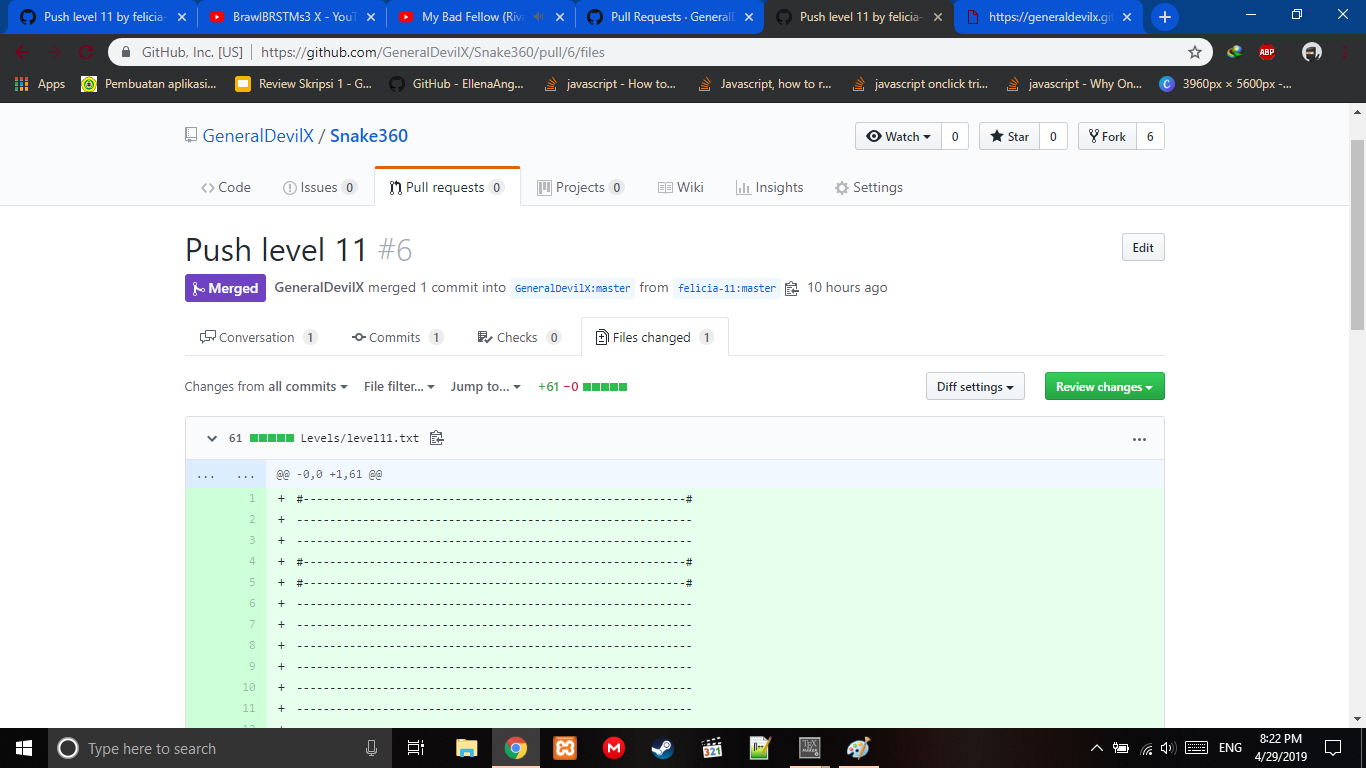
\includegraphics[scale=0.4]{pullReq4}  
		\caption[Tampilan hasil \textit{pull request} milik penguji 4]{Tampilan hasil \textit{pull request} milik penguji 4}
		\label{fig:pullReq4} 
	\end{figure}
	
	\begin{figure}[H]
		\centering  
		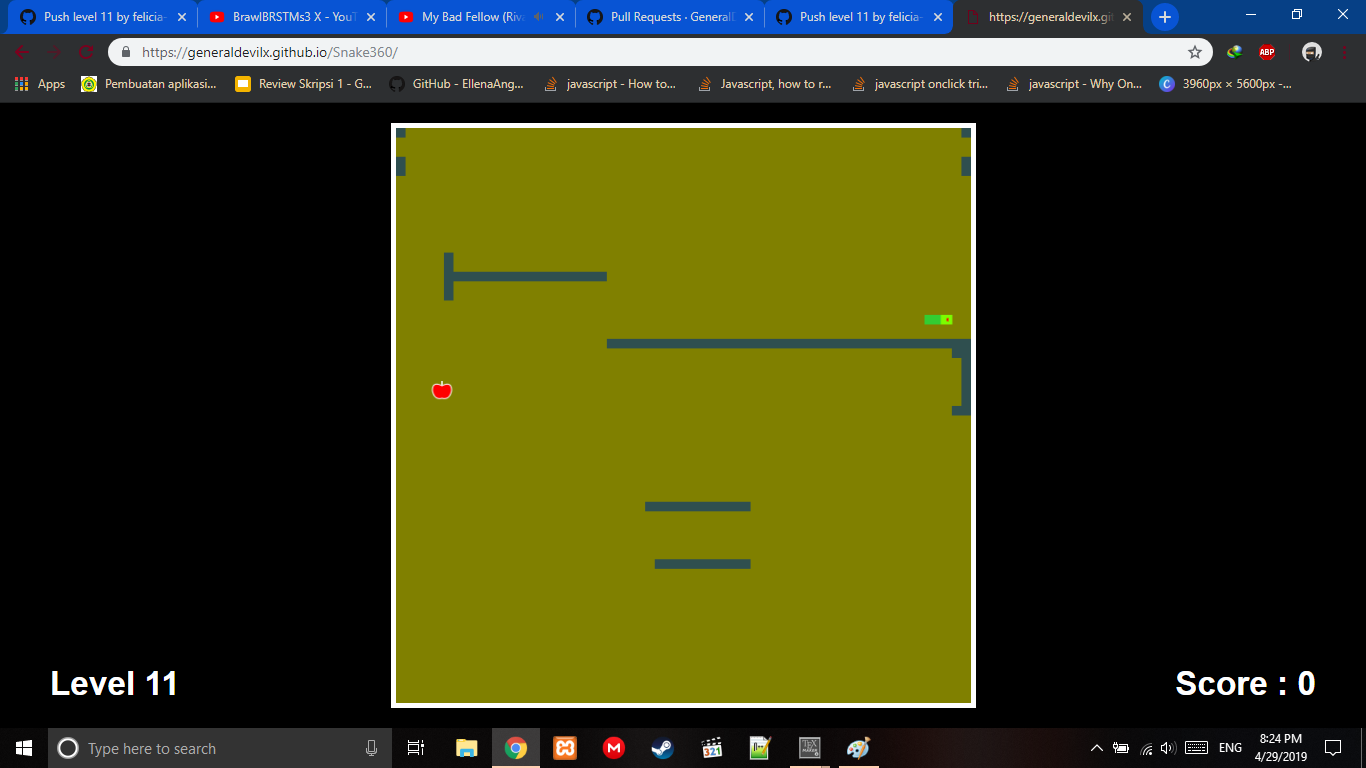
\includegraphics[scale=0.4]{pengujian4}  
		\caption[Tampilan pengujian labirin yang dibuat oleh penguji 4]{Tampilan pengujian labirin yang dibuat oleh penguji 4}
		\label{fig:pengujian4} 
	\end{figure}
	
	\item Penguji 5 : tegarmuhammad3775\\
	Penguji 5 berhasil menambahkan labirin \textit{level} 12 dengan menggunakan \textit{pull request} seperti yang terlihat pada Gambar~\ref{fig:pullReq5}. Link untuk file teks yang dibuat penguji 5 : \url{https://github.com/GeneralDevilX/Snake360/pull/5/files}. Labirin yang dibuat oleh penguji 5 sudah sesuai ketentuan membuat labirin pada \textit{file readme} sehingga tampilan menjadi seperti pada Gambar~\ref{fig:pengujian5}.
	
	\begin{figure}[H]
		\centering  
		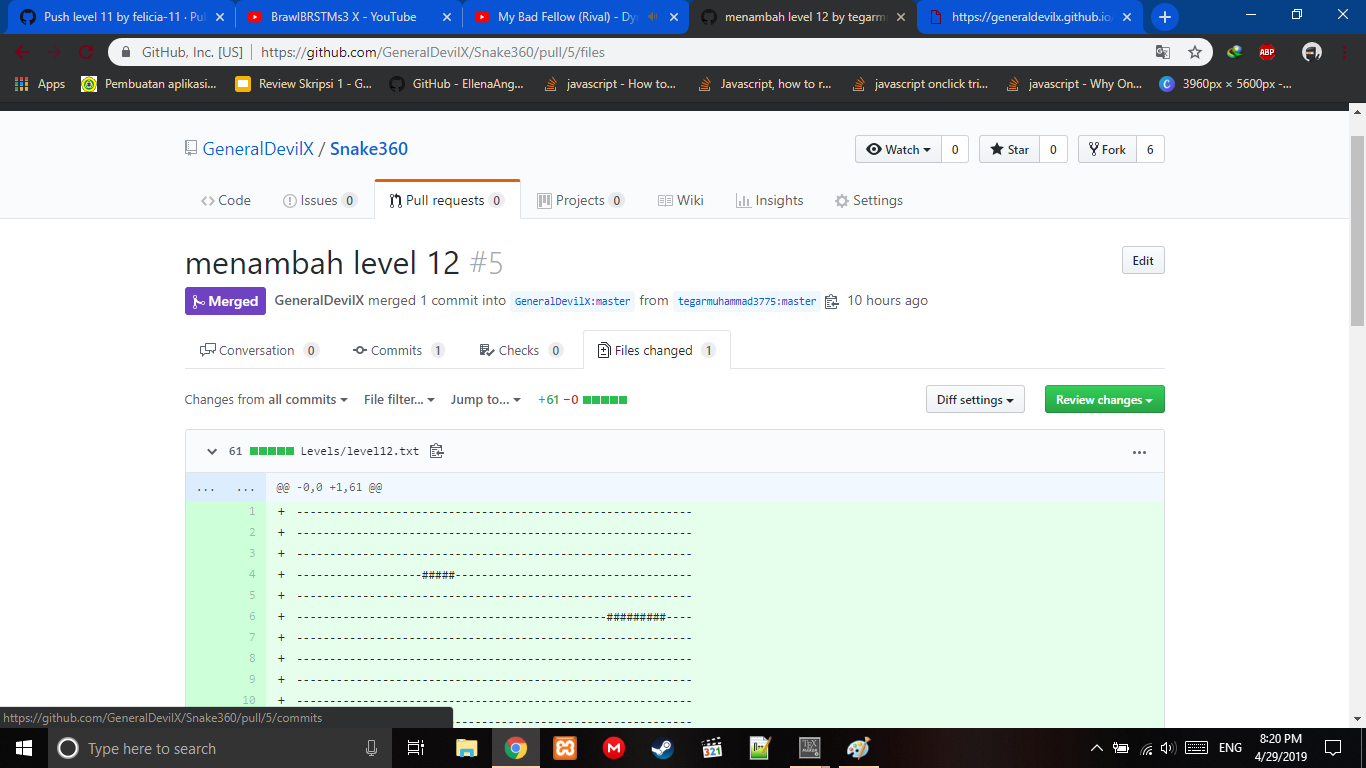
\includegraphics[scale=0.4]{pullReq5}  
		\caption[Tampilan hasil \textit{pull request} milik penguji 5]{Tampilan hasil \textit{pull request} milik penguji 5}
		\label{fig:pullReq5} 
	\end{figure}
	
	\begin{figure}[H]
		\centering  
		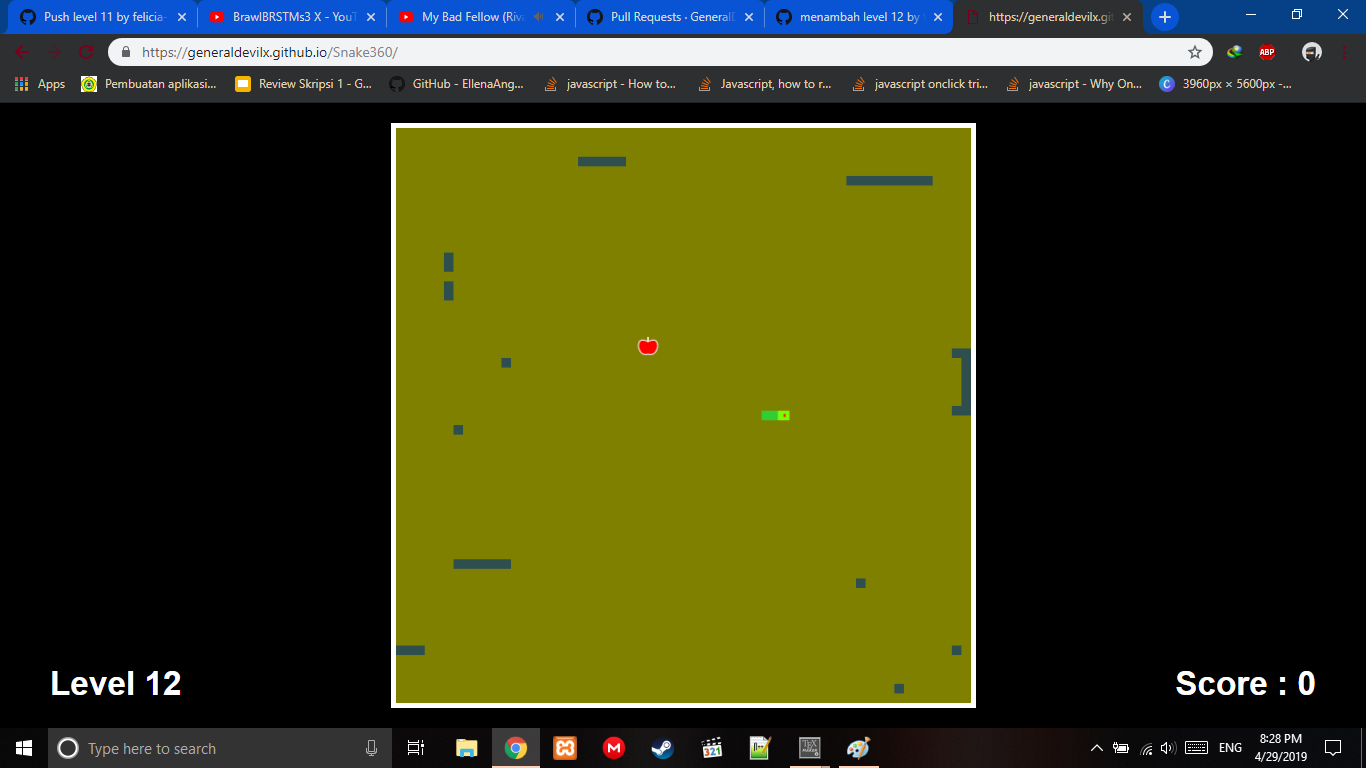
\includegraphics[scale=0.4]{pengujian5}  
		\caption[Tampilan pengujian labirin yang dibuat oleh penguji 5]{Tampilan pengujian labirin yang dibuat oleh penguji 5}
		\label{fig:pengujian5} 
	\end{figure}
\end{enumerate}